\chapter{Considerações Gerais}
\label{cap:02}

\section{O que é um jogo?}

Segundo o designer de jogos \citeauthorandyear{Crawford1997}, para compreender os jogos e seu design, deve-se primeiramente definir o que se quer representar com a palavra "jogo", a qual ele define como sendo um sistema fechado que representa subjetivamente um subconjunto da realidade. Essa afirmação descreve um jogo como algo completo e autossuficiente, com regras bem definidas que determinam seu funcionamento.

Além disso, o autor identifica quatro elementos fundamentais presentes em todos os jogos. O primeiro é a representação, pois considera que todo jogo sempre reflete, de alguma maneira, aspectos da realidade, mesmo que de forma abstrata ou fantasiosa. O segundo é a interação, pois os jogadores influenciam o jogo ao tomarem decisões. O terceiro é o conflito, que se manifesta por meio de desafios e competição. Por fim, há a segurança, já que as consequências do jogo raramente impactam a realidade.


Já \citeauthorandyear{Suits1978}, filósofo canadense conhecido por seu trabalho sobre a natureza dos jogos, apresenta uma definição mais voltada para o ato de jogar, na qual determina que jogar um jogo é se envolver voluntariamente a uma atividade para alcançar um estado específico, aceitando seguir regras limitantes. Ele também introduz o conceito de \textit{lusory attitude}, que consiste nos jogadores se submeterem a desafios desnecessários para tornar o jogo possível. 



\citeauthorandyear{Crawford1997} define os tipos distintos de jogos, caracterizados a seguir.



\subsection{Jogos de Tabuleiro}

Primeiramente, temos os jogos de tabuleiro, que consistem em uma superfície dividida em setores, os quais são ocupados por um conjunto de peças que, nas configurações comuns, estão diretamente associadas aos jogadores, que as movimentam pelo tabuleiro com o objetivo de capturar as peças do adversário. Um exemplo popular desse tipo de jogo é o Xadrez, que se destaca como um dos jogos de estratégia mais clássicos e influentes, representando bem a essência dos jogos de tabuleiro.

Na Figura~\ref{fig:xadrez}, é ilustrado um tabuleiro de Xadrez com suas peças no começo de uma partida.


\FloatBarrier
\begin{figure}[!htbp]
	\centering
	\caption{Tabuleiro de Xadrez e suas peças}
	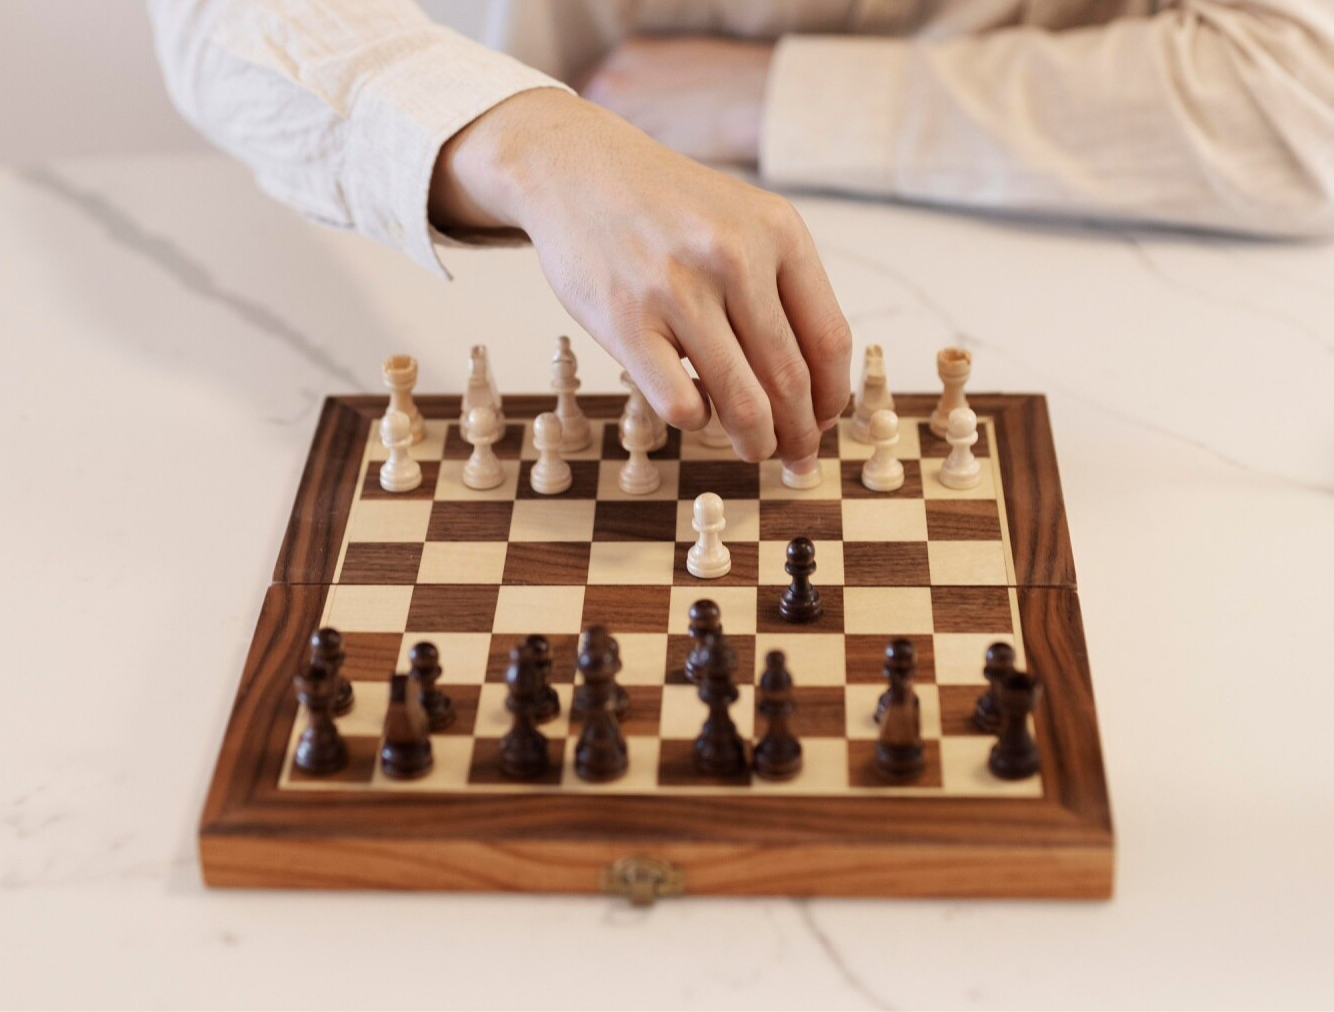
\includegraphics[width=0.7\linewidth]{imagens/Xadrez.png}
	\\\textbf{Fonte:} Freepik
	\label{fig:xadrez}
\end{figure}
\FloatBarrier

\subsection{Jogos de Cartas}

Uma segunda classe de jogos são os jogos de carta, que utilizam um baralho composto por 52 cartas, divididos entre quatro naipes e treze fileiras. O uso do baralho varia conforme o objetivo do jogo, e uma das razões pelas quais os jogos de cartas são tão fascinantes é seu equilíbrio entre sorte e habilidade, diferente dos jogos totalmente aleatórios, como os dados, ou puramente estratégicos, como o xadrez \cite{Parlett1990}.


Segundo \citeauthorandyear{Parlett1990} as cartas possuem uma característica dupla que influencia diretamente a dinâmica dos jogos: a aleatoriedade, que ocorre porque são embaralhadas antes do jogo, e o sigilo, já que apenas o jogador que as possui pode ver seu valor. A questão de sorte nos jogos de cartas está frequentemente ligada à probabilidade, permitindo assim utilizar cálculos matemáticos para prever e influenciar resultados ao longo das partidas. 

Na Figura~\ref{fig:cartas} são apresentadas as cartas presentes em um baralho.


\FloatBarrier 
\begin{figure}[!htbp]
	\centering
	\caption{Cartas de um baralho}
	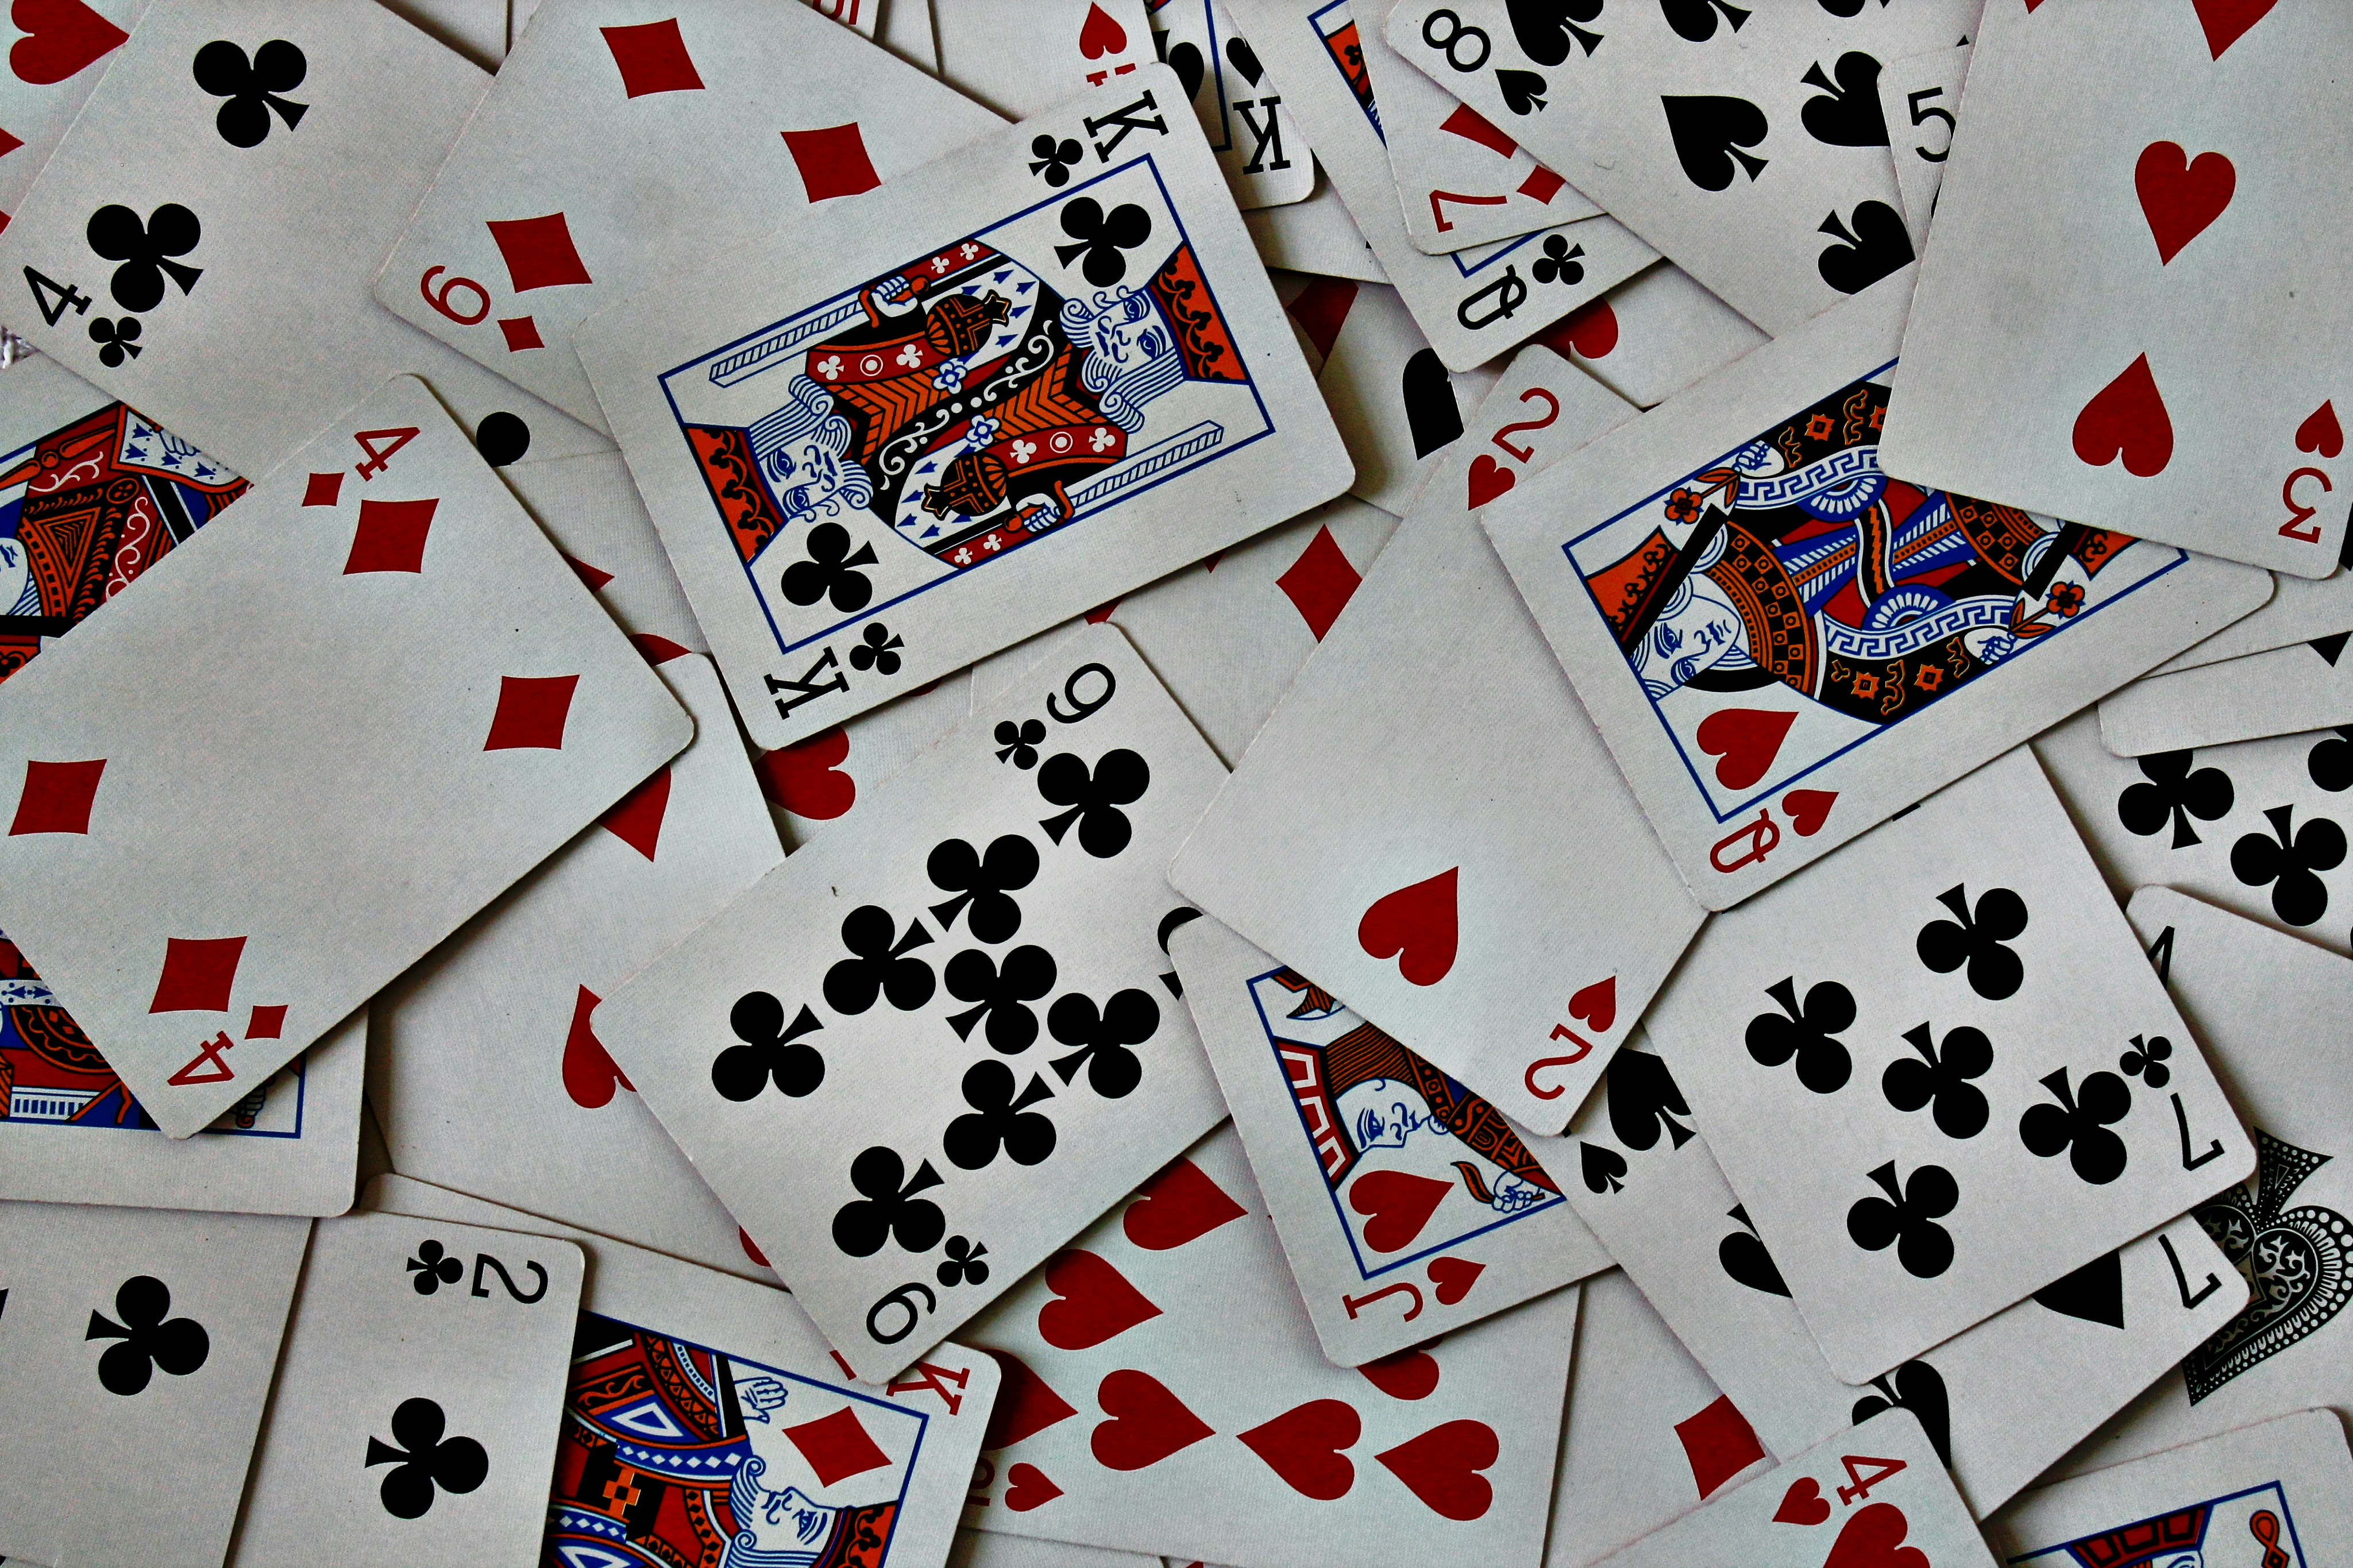
\includegraphics[width=0.7\linewidth]{imagens/Cartas.jpg}
	\\\textbf{Fonte:} https://unsplash.com/pt-br/fotografias/uma-pilha-de-cartas-de-baralho-sentadas-umas-em-cima-das-outras-P787-xixGio
	\label{fig:cartas}
\end{figure}
\FloatBarrier


\subsection{Jogos Atléticos}


Há também os jogos atléticos, uma das formas mais tradicionais de jogos, que destaca a destreza física em detrimento das habilidades mental e possuem regras que especificam estritamente as ações que o jogador pode ou não realizar. Tais jogos estão em uma linha tênue com as competições atléticas, sendo distinguidos pelo grau de interação entre os jogadores \cite{Crawford1997}. Na Figura~\ref{fig:futebol} há um exemplo de jogo atlético, o futebol.


\FloatBarrier 
\begin{figure}[!htbp]
	\centering
	\caption{Jogo de futebol}
	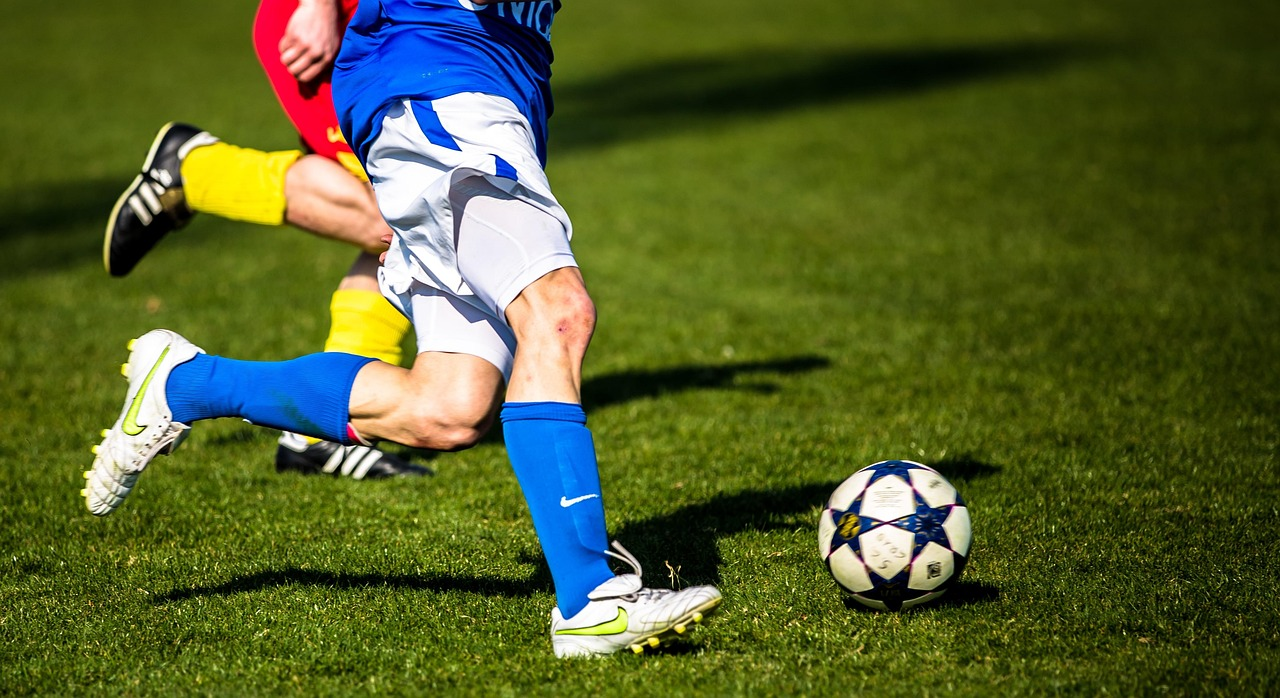
\includegraphics[width=0.7\linewidth]{imagens/futebol.jpg}
	\\\textbf{Fonte:} https://pixabay.com/pt/photos/futebol-duelo-grama-bola-esportes-1331838/
	\label{fig:futebol}
\end{figure}
\FloatBarrier



\subsection{Jogos Digitais}


Por fim, temos os jogos digitais, os mais populares atualmente e a categoria central deste trabalho. Esses jogos se adequam a diferentes tipos de computadores e plataformas, incluindo máquinas dedicadas, como os fliperamas, consoles domésticos, computadores pessoais e dispositivos portáteis, como o \textit{Nintendo DS} ou até mesmo os celulares \cite{Crawford1997}.


\section{Tipos de Jogos Eletrônicos}

Segundo a definição de \citeauthorandyear{Juul2005}, pesquisador dinamarquês reconhecido na área de \textit{game studies}, os jogos eletrônicos são definidos como uma combinação de regras reais inseridas em mundos fictício, com os quais os jogadores interagem. Essa interação não se limita apenas às mecânicas dos jogos; ela se manifesta em diversos aspectos, incluindo seu design, bem como a forma que os jogos são interpretados, utilizados e discutidos.

No entanto, essa definição desconsidera aspectos culturais nos quais o jogo está inserido, focando apenas na estrutura interna do jogo. E a partir disso, \citeauthorandyear{Apperley2006}, teórico da mídia digital e pesquisador dos estudos de jogos, propõe uma abordagem alternativa, categorizando os videogames com base em como eles são jogados e recebidos. Essa proposta compreende os jogos a partir das práticas sociais e culturais, enfatizando a experiência prática e situada do jogador.

A categorização dos videogames de \citeauthorandyear{Apperley2006} será apresentada a seguir.


\subsection{Simulação}

Embora todos os jogos sejam, de certa forma, simulações, os jogos de simulação buscam representar claramente uma atividade do mundo real, sendo relacionadas a esportes, voos e direção, ou até mesmo simular a dinâmica de cidades e vilarejos. A maior parte desses jogos se encaixam na noção de remediação, pois sua jogabilidade é reaproveitada de atividades relativamente comuns ou representadas nas mídias. Um exemplo popular é o jogo \textit{Euro Truck Simulator}, que simula a direção de um caminhão, apresentada na Figura~\ref{fig:simulacao}.


\FloatBarrier 
\begin{figure}[!htbp]
	\centering
	\caption{\textit{Euro Truck Simulator}}
	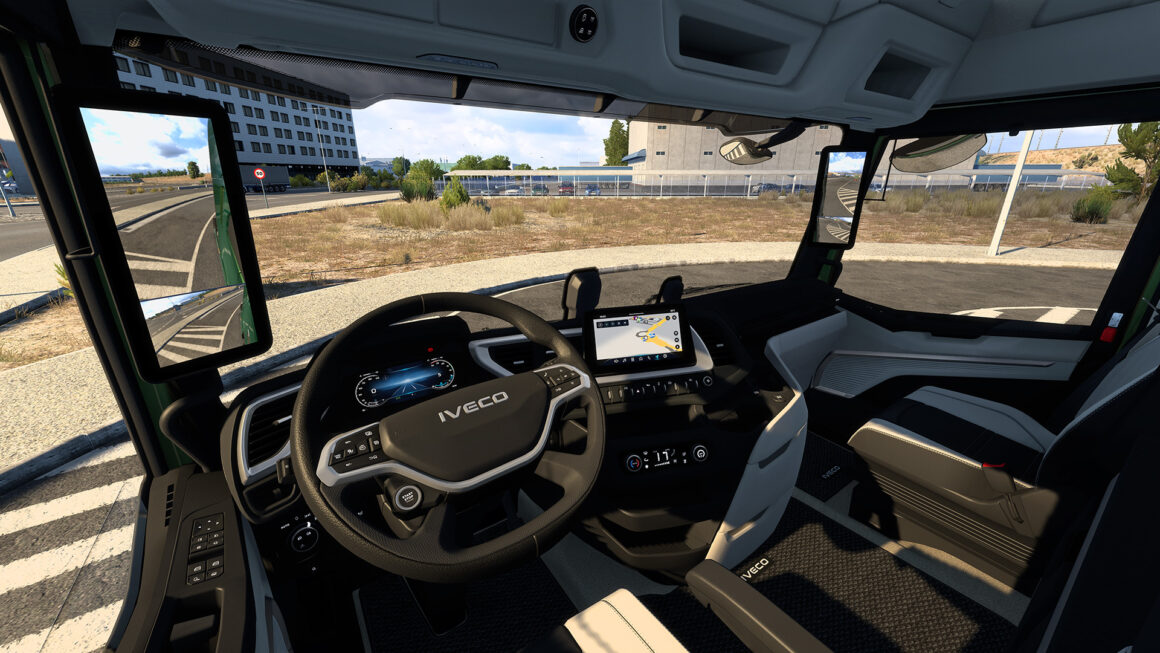
\includegraphics[width=0.7\linewidth]{imagens/EuroTruck.jpg}
	\\\textbf{Fonte:}https://estradao.estadao.com.br/caminhoes/caminhao-pesado-iveco-s-way-estreia-no-euro-truck-simulator-2/ 
	
	\label{fig:simulacao}
\end{figure}
\FloatBarrier


\subsection{Estratégia}

Os jogos de estratégia são caracterizados pelo planejamento e pela tomada de decisões táticas. Geralmente são divididos em dois subgêneros: a estratégia em tempo real (RTS) e baseada em turnos (TBS). Ambos possuem uma estética semelhante, sendo tendentes a um conceito fotorrealista. Tais jogos priorizam a gestão de recursos, o pensamento analítico e a adaptação estratégica, exigindo, assim, uma atenção profunda do jogador. Um exemplo de TBS é o jogo \textit{Teamfight Tactics (TFT)} apresentado na Figura~\ref{fig:tactics}.

\FloatBarrier 
\begin{figure}[!htbp]
	\centering
	\caption{\textit{Teamfight Tactics (TFT)}}
	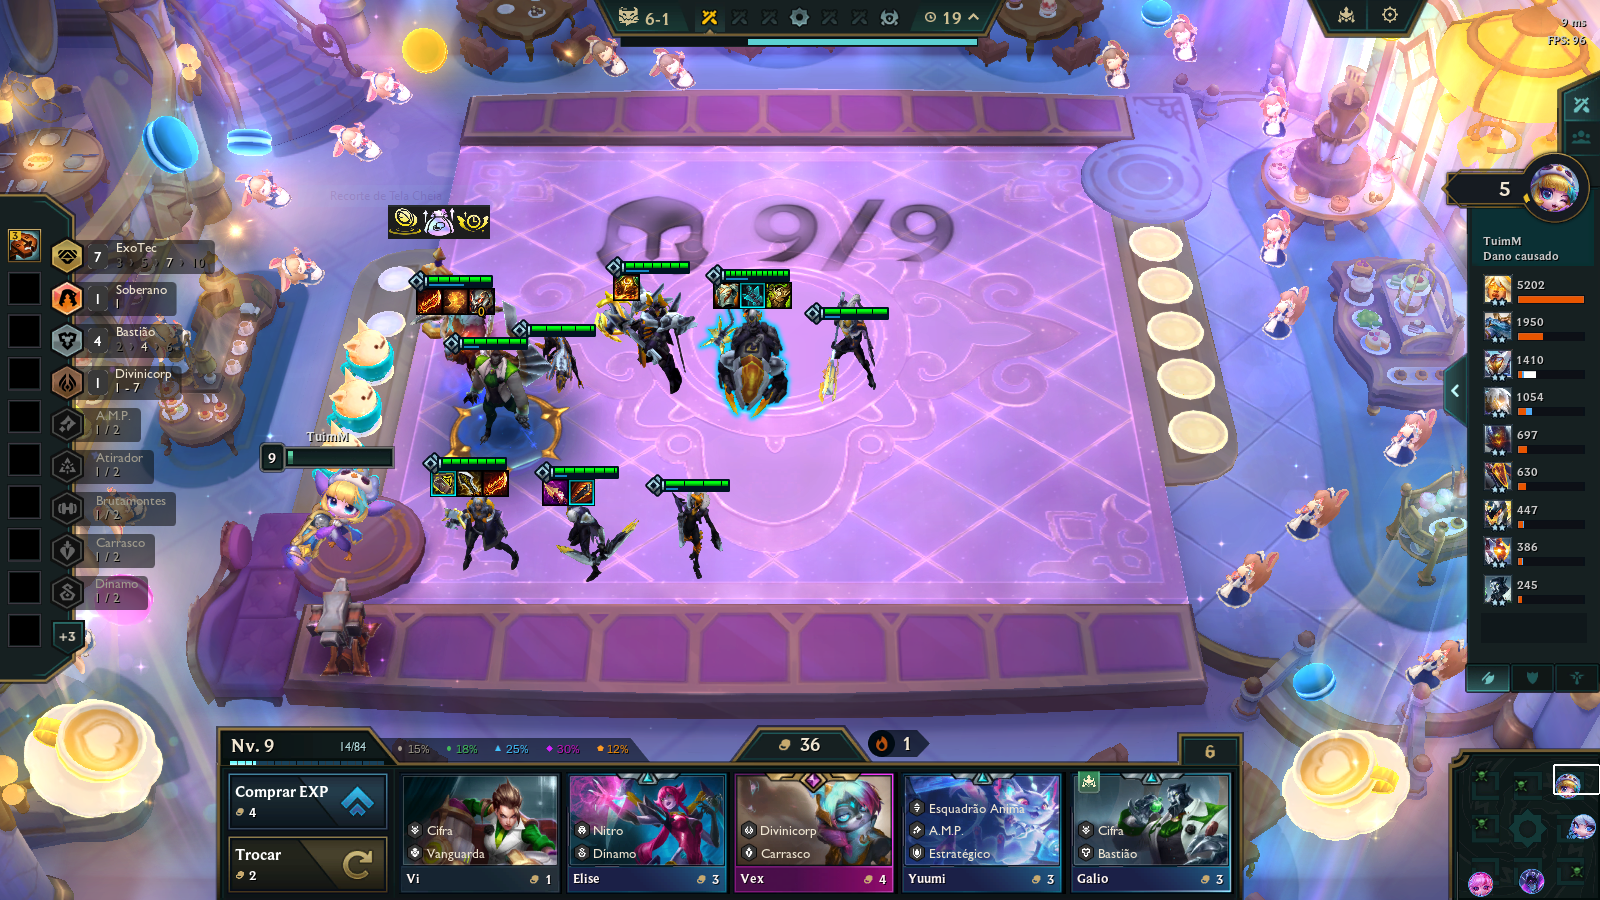
\includegraphics[width=0.7\linewidth]{imagens/tft3.png}
	\\\textbf{Fonte:} Elaborada pelo autor
	
	\label{fig:tactics}
\end{figure}
\FloatBarrier


\subsection{Ação}

Assim como os jogos de estratégia, os jogos de ação também podem ser divididos em dois subgêneros: jogos de tiro em primeira pessoas, conhecidos como FPS (\textit{First Person Shooters}), nos quais a câmera simula a própria visão do jogador, e jogos em terceira pessoa, que representam o personagem totalmente visível na tela, geralmente visto por trás. Tais jogos priorizam a agilidade, precisão e o tempo de reação do jogador, oferecendo experiências intensas e dinâmicas. Um FPS popular é o jogo \textit{Valorant} apresentado na Figura~\ref{fig:vava}.


\FloatBarrier 
\begin{figure}[!htbp]
	\centering
	\caption{\textit{Valorant}}
	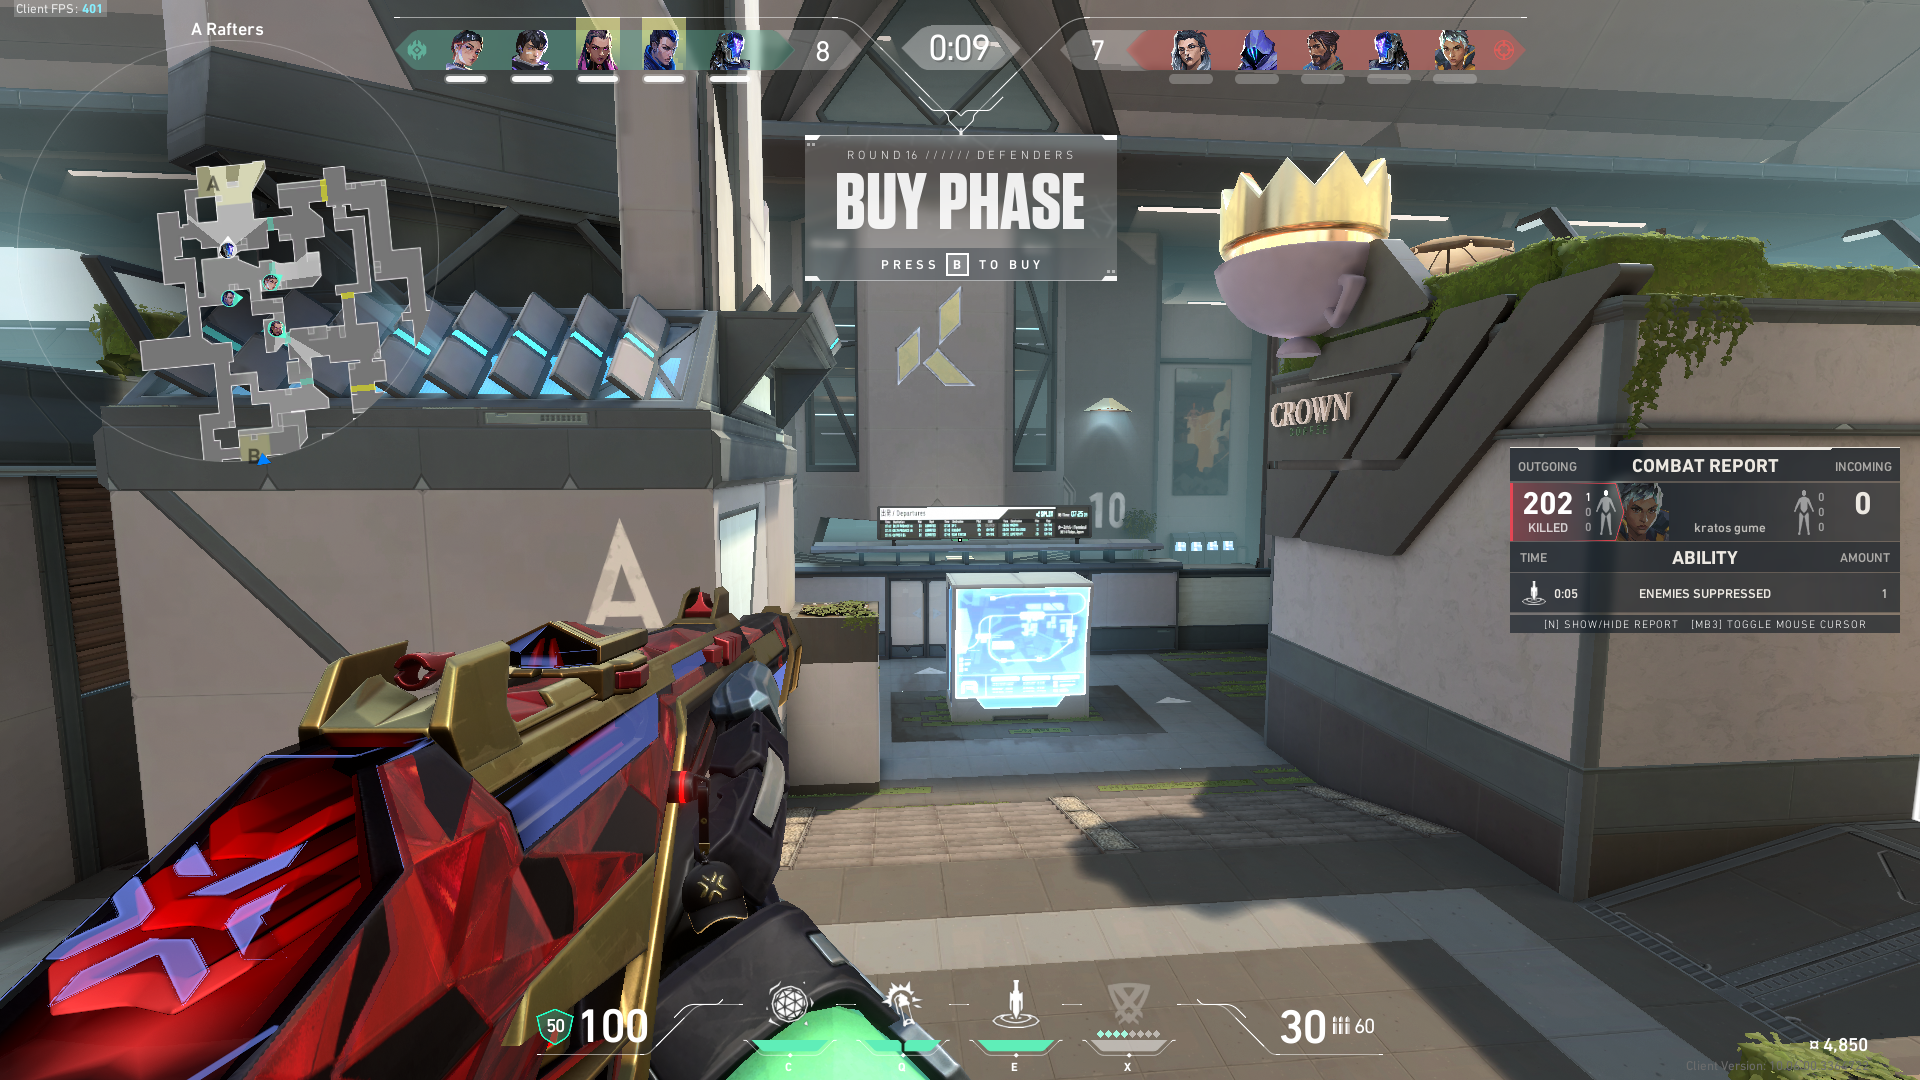
\includegraphics[width=0.7\linewidth]{imagens/valorant.png}
	\\\textbf{Fonte:} Elaborada pelo autor
	
	\label{fig:vava}
\end{figure}
\FloatBarrier


\subsection{\textit{Role-playing}}

Nos jogos de \textit{Role-playing}, ou RPGs, os jogadores interpretam seus personagens em mundos fictícios, narrando suas ações a um mestre, o qual conduz os resultados dessas ações. Originados do clássico  \textit{Dungeons and Dragons} na década de 1970 \cite{Mason2004}, esse jogos evoluíram para versões digitais, mantendo elementos como a progressão de personagens, porém agora limitando a improvisação e focando em desafios mecânicos e uma narrativa mais centrada.

\section{Tecnologias para Desenvolvimento de Jogos} 

(dar contextualização para a explicação da engine...)

De acordo com a definição de \citeauthorandyear{CluaBittencourt2005}, uma \textit{engine}, ou motor gráfico, é uma ferramenta essencial no desenvolvimento de jogos, responsável por executar diversas funcionalidades técnicas. Entre elas estão o \textit{hardware} gráfico, o controle dos modelos a serem renderizados e o tratamento das entradas de dados do jogador. Além disso, ela lida com os processos básicos que garantem o funcionamento adequado do jogo. 

\subsection{Godot}

A \textit{Godot} é uma \textit{engine} de código aberto, totalmente independente e conduzida pela comunidade, com o apoio da fundação \textit{Godot Foundation}. Trata-se de uma \textit{engine} multiplataforma que suporta criação de jogos 2D e 3D, oferece um conjunto abrangente de ferramentas integradas, proporcionando aos desenvolvedores uma maior praticidade. Além disso, ela promove uma facilidade de exportação para diversas plataformas, como sistemas \textit{desktop}, dispositivos móveis e consoles  \cite{GodotDocs2024}.

De acordo com o desenvolvedor de jogos e escritor \citeauthorandyear{Bradfield2018}, a Godot é uma \textit{engine} moderna e completa, tendo como diferencial o fato de a ferramenta ser totalmente gratuita e distribuída sob a licença MIT, a qual assegura aos desenvolvedores liberdade total sobre seus projetos. Tal atrativo distingue a \textit{Godot} das demais \textit{engine}, as quais estabelecem restrições contratuais ou cobranças sobre a porcentagem dos lucros obtidos com os jogos criados.


Além desses benefícios, a \textit{Godot} possui sua própria linguagem de programação, a  \textit{GDScript}. Desenvolvida especialmente para a \textit{engine}, ela oferece uma sintaxe simples, sendo semelhante à do Python, e permite uma integração total com o editor. A \textit{GDScript} foi criada com foco em desempenho e produtividade, evitando limitações comuns encontradas em outras linguagens de uso geral no desenvolvimento de jogos.\cite{GodotDocs2024}.

Na Figura~\ref{fig:godot} é apresentado a interface da \textit{engine Godot}.

\FloatBarrier 
\begin{figure}[!htbp]
	\centering
	\caption{\textit{Interface Godot}}
	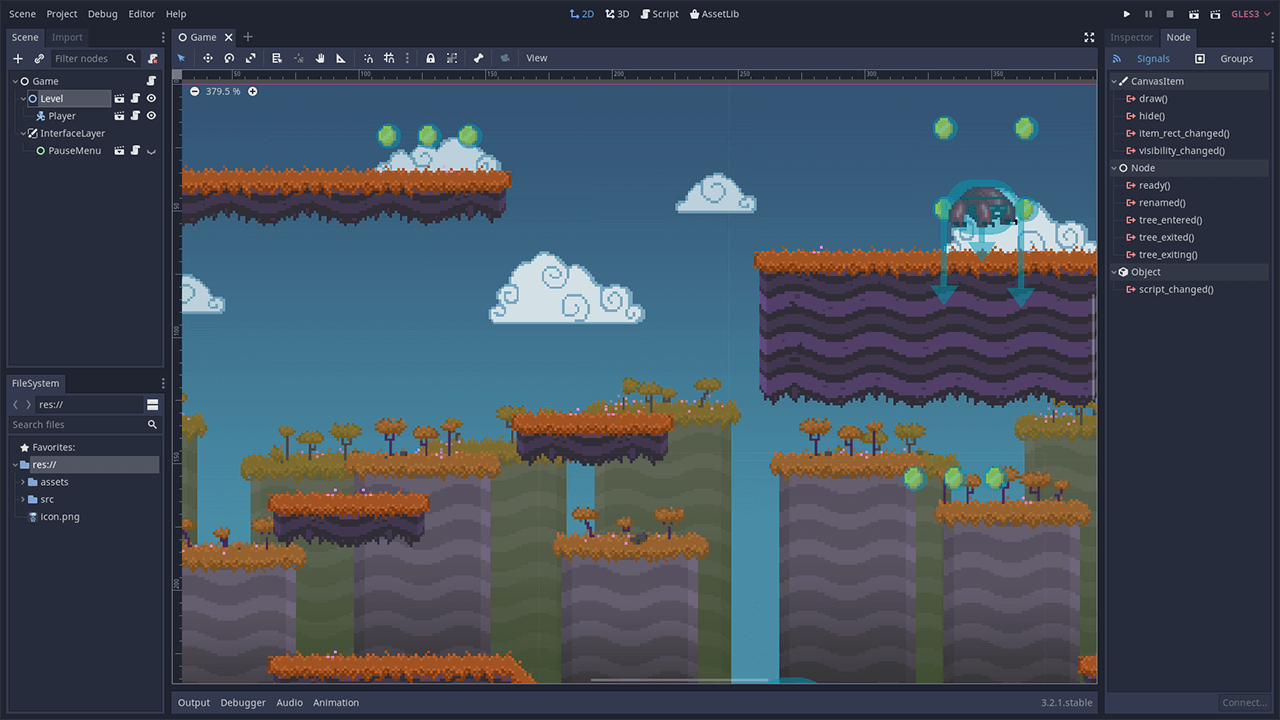
\includegraphics[width=0.7\linewidth]{imagens/godot-editor-01.png}
	\\\textbf{Fonte:} https://videogamewarlock.com/godot-engine-desenvolva-games-com-liberdade/
	
	\label{fig:godot}
\end{figure}
\FloatBarrier


\subsection{Unity}

A \textit{Unity} é um motor de jogos multiplataformas amplamente utilizado no desenvolvimento de jogos 2D e 3D, assim como na criação de visualizações e simulações interativas. É considerada um dos motores mais populares entre os desenvolvedores, devido sua facilidade de uso, flexibilidade e eficiência. Seu ambiente de desenvolvimento disponibiliza diversos recursos integrados, como o \textit{Adaptive Performance} e o suporte à programação em C\#, que possibilitam a criação de jogos com alto desempenho e qualidade \cite{Hussain2020}.

A empresa \textit{Unity Technologies } é a responsável pelo desenvolvimento da \textit{Unity}, cuja primeira versão foi lançada em 2005, durante a conferência da \textit{Apple}. Inicialmente, essa versão era voltada somente para o desenvolvimento no sistema OS X, visando tornar a criação de jogos mais acessível. Atualmente, a \textit{Unity} evoluiu e oferece suporte para certa de 27 plataformas  incluindo dispositivos móveis, desktops, consoles, navegadores e realidade virtual \cite{Smid2017}.

Na Figura~\ref{fig:unity} é apresentado a interface da \textit{engine Unity}.

\FloatBarrier 
\begin{figure}[!htbp]
	\centering
	\caption{\textit{Interface Unity}}
	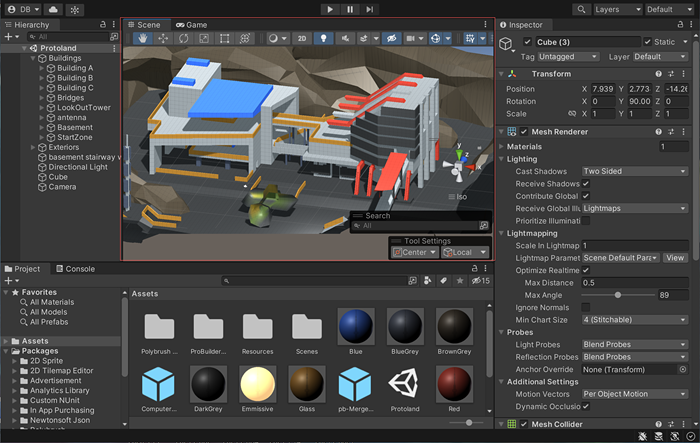
\includegraphics[width=0.7\linewidth]{imagens/unity.png}
	\\\textbf{Fonte:} https://docs.unity3d.com/Manual/UsingTheSceneView.html 
	\label{fig:unity}
\end{figure}
\FloatBarrier



\subsection{Unreal Engine}

A \textit{Unreal Engine} é um motor gráfico desenvolvido pela empresa \textit{Epic Games} e, atualmente, é considerada a principal \textit{engine} para visualizações realistas, e a criação de vegetação e terrenos. É a \textit{engine} mais indicada para projetos grandes e, embora possua suporte para \textit{IOS} e \textit{Android}, não é a mais recomendada para jogos \textit{mobile}. Um de seus maiores diferencias é o sistema \textit{Blueprint}, uma ferramenta visual de lógica composta por grafos conectados através de blocos, substituindo a necessidade de scripts tradicionais \cite{Smid2017}.

Também de acordo com o acadêmico \citeauthorandyear{Smid2017}, a \textit{Unreal Engine} utiliza da linguagem de programação C++, tanto para implementação dos jogos quanto para o desenvolvimento de seu código-fonte aberto, proporcionando assim um grande controle sobre o sistema para os usuários. Além disso, sua tecnologia de renderização é muito eficaz, possuindo efeitos de pós-processamento rápidos com diversos recursos integrados. A \textit{engine} também dispõe de um editor para a criação de  materiais personalizados, e ferramentas para otimização e depuração visual.

(...)

\subsection{Game Maker}	

\textit{text}


\section{Trabalhos Correlatos}

\subsection{Speedy Dungeon}

Texto...

\subsection{Luxos Adventure}

Texto...

\subsection{Trabalho 3}

Texto...
